\documentclass[10pt,landscape,a4paper]{article}
\usepackage[utf8]{inputenc}
\usepackage[nosf]{kpfonts}
\usepackage[t1]{sourcesanspro}

% For the multiple columns in the cheat sheet
\usepackage{multicol}

% Set the margins of the paper
\usepackage[margin=1mm]{geometry}

% To use colours
\usepackage{xcolor}

% To typeset small fonts
\usepackage{microtype}

% To have easier typesetting of units
\usepackage{siunitx}

% To include graphics
\usepackage{graphicx}

\graphicspath{ {./images/} }

\let\bar\overline

\definecolor{myblue}{cmyk}{1,.72,0,.38}

\everymath\expandafter{\the\everymath \color{myblue}}
\everydisplay\expandafter{\the\everydisplay \color{myblue}}

\renewcommand{\baselinestretch}{.8}
\pagestyle{empty}

\makeatletter
\renewcommand{\section}{\@startsection{section}{1}{0mm}%
  {.2ex}%
  {.2ex}%x
  {\color{myblue}\sffamily\small\bfseries}}
\renewcommand{\subsection}{\@startsection{subsection}{1}{0mm}%
  {.2ex}%
  {.2ex}%x
  {\sffamily\bfseries}}


\makeatother
\setlength{\parindent}{0pt}

\begin{document}
\small
\begin{multicols*}{5}
  \raggedcolumns


  \section{Linkages}

  Degrees of freedom: \\
  \(DoF = 3(n_L - 1) - 2n'_J - n''_J\)

  4-bar linkage condition: \\
  \(L_{max} \le L_{min} + L_a + L_b\)

  Grashof condition: \\
  \(L_{max} + L_{min} \le L_a + L_b\)

  Actual number of joints \(=\) Number of links attached to joint \(- 1\)

  \subsection{Types of linkages}
  Crank-rocker: Shortest link next to the fixed link \\
  Drag-link: Shortest link is the fixed link \\
  Double rocker: Shortest link is opposite the fixed link \\
  Change-point or crossover-position: All links are collinear \\
  Triple rocker: Non-Grashof linkage, none of the links makes a \(\qty{360}{\degree}\) rotation

  \section{Gears}

  Terminology: \\
  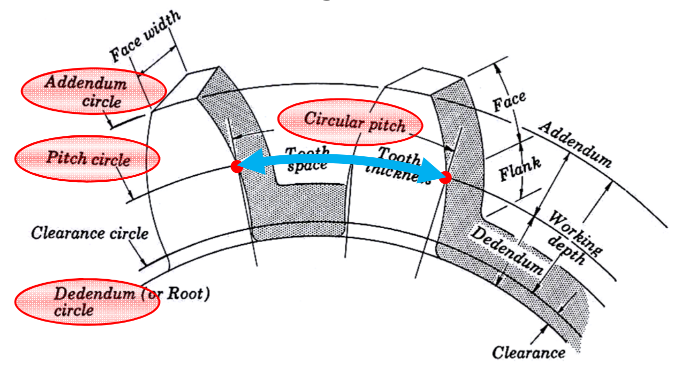
\includegraphics[width=\linewidth]{spur-gear-terminology}

  Module: \\
  \(m = \frac{d_p}{N}\)

  Circular pitch: \\
  \(p_c = \pi \frac{\pi d_p}{N} = \pi m\)

  Diametral pitch (\(P_d\)): \\
  \(\frac{1}{P_d} = \frac{m}{25.4}\)

  Pitch circle radius: \\
  \(r = \frac{mN}{2}\)

  Tooth thickness: \\
  \(t = \frac{\pi}{2}\)

  Addendum: \\
  \(a = m\)

  Velocity ratio: \\
  \(r_v = \frac{\omega_2}{\omega_1} = \frac{RPM_2}{RPM_1} = \frac{r_1}{r_2} = \frac{N_1}{N_2}\)

  Centre distance: \\
  \(c = \frac{d_{p1} + d_{p2}}{2} = \frac{m(N_1 + N_2)}{2} = \frac{N_1 + N_2}{2P_d}\)

  Base-circle radius: \\
  \(r_b = r \cos \phi\)

  Base pitch: \\
  \(p_b = m \pi \cos \phi = \frac{\pi}{P} \cos \phi\)

  Contact ratio: \\
  \(C.R. = \frac{\sqrt{(r_2 + a_2)^2 - r_2^2 \cos^2 \phi} - r_2 \sin \theta}{p_b} + \frac{\sqrt{(r_1 + a_1)^2 - r_1^2 \cos^2 \phi} - r_1 \sin \theta}{p_b}\)

  Power: \\
  \(P = \omega T\)

  Tangential force on a gear: \\
  \(F_t = \frac{T}{r} = \frac{2T}{mN}\)

  Radial force on a gear: \\
  \(F_r = F_t \tan \phi\)

  \subsection{Avoiding interference}

  Condition: \\
  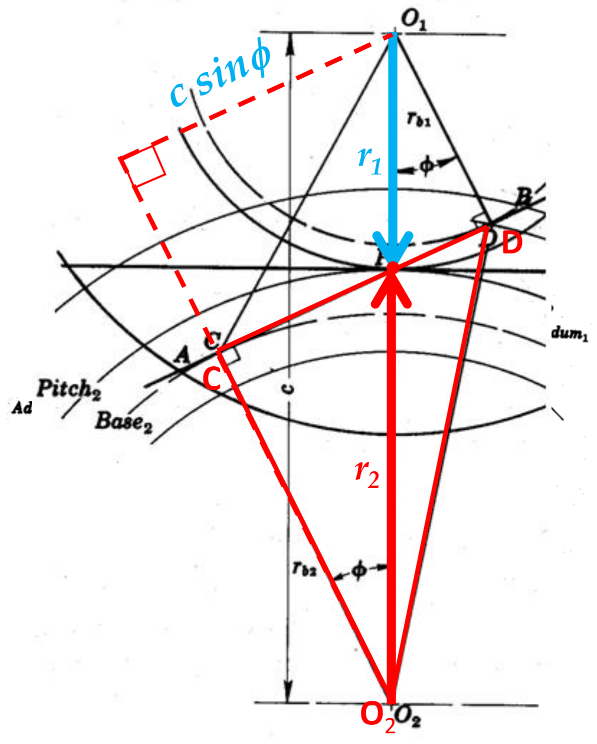
\includegraphics[width=\linewidth]{avoiding-interference-diagram}
  \(r_1 + a_1 \le \sqrt{r_1^2 \cos^2 \phi + c^2 \sin^2 \phi}\) \\
  \(r_2 + a_2 \le \sqrt{r_2^2 \cos^2 \phi + c^2 \sin^2 \phi}\)

  Pinion and rack condition: \\
  \(N \ge \frac{2k}{\sin^2 \phi}\)

  \subsection{Gear trains}

  Formula: \\
  \(\frac{\text{Target gear, } n_T}{\text{Driving gear, } n_D} = \frac{\text{Driving gear}}{\text{Driven gear}}\)

  Planetary gear chains: \\
  \(\frac{n_T - n_c}{n_D - n_c} = \left(-\frac{N_1}{N_2} \right) \left(- \frac{N_3}{N_4} \right) \cdots\)

  Getting the gear ratio: \\
  \(\Diamond\) \(-\) for external gear \\
  \(\Diamond\) \(+\) for internal gear

  \subsection{Reverted gear trains}

  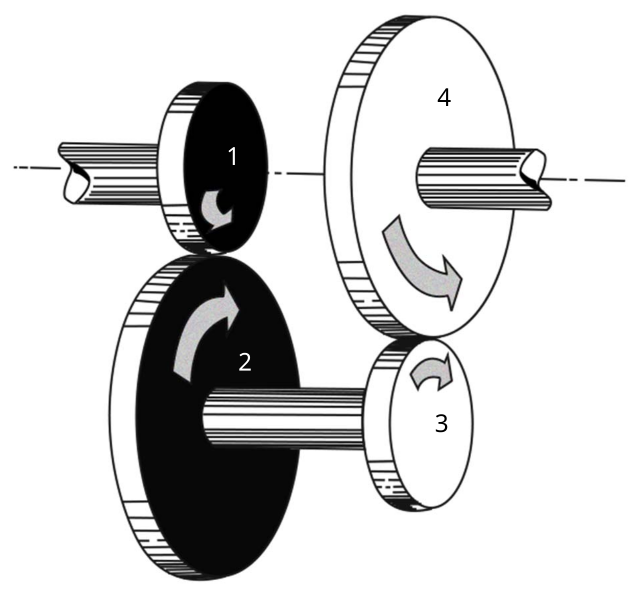
\includegraphics[width=0.8\linewidth]{reverted-gear-train-image} \\

  External gears: \\
  \(r_1 + r_2 = r_3 + r_4\) \\
  External to internal gears: \\
  \(r_{internal_1} - r_{external_1} = r_{internal_2} - r_{external_2}\)

  \section{Vector loop equations}
  \(\Diamond\) Set up a global reference frame. \\
  \(\Diamond\) Assign a direction vector to all links. \\
  \(\Diamond\) Ensure the direction vectors all form a loop and write an equation based on that. \\
  \(\Diamond\) Split the vectors into their sine and cosine components. \\
  \(\Diamond\) Figure out which vectors don't change their length or direction and set them as constants. \\
  \(\Diamond\) Differentiate to find the velocity and acceleration if necessary.

  \section{Cam motion}

  Uniform motion: \\
  \(s = \frac{L}{\beta} \theta\) \\
  \(\dot{s} = \frac{L}{\beta} \dot{\theta}\) \\
  \(\ddot{s} = \frac{L}{\beta} \ddot{\theta}\) \\
  \(\dddot{s} = \frac{L}{\beta} \dddot{\theta}\) \\

  Parabolic motion: \\
  1st parabola: \(s = \frac{2L}{\beta^2} \theta^2\) \\
  2nd parabola: \(s = - L + \frac{4L}{\beta} \theta - \frac{2L}{\beta^2} \theta^2\)

  Simple harmonic motion: \\
  \(s = \frac{L}{2} \left(1 - \cos \frac{\pi \theta}{\beta} \right)\) \\
  \(\dot{s} = \frac{\pi L \omega}{2\beta} \sin \frac{\pi \theta}{\beta}\) \\
  \(\ddot{s} = \frac{L}{2} \left(\frac{\pi L \omega}{2 \beta} \right)^2 \cos \frac{\pi \theta}{\beta}\) \\
  \(\dddot{s} = \frac{L}{2} \left(\frac{\pi L \omega}{2 \beta} \right)^3 \sin \frac{\pi \theta}{\beta}\)

  Cycloidal motion: \\
  \(s = L \left(\frac{\theta}{\beta} - \frac{1}{2\pi} \sin \left(\frac{2\pi\theta}{\beta} \right) \right)\)

  Rise and return: \\
  \(\Diamond\) During rise, replace \(\theta\) with \(\theta - \theta_i\) \\
  \(\Diamond\) During return, replace \(\theta\) with \(\theta_e - \theta\)

  \section{Cam profile}

  Cam profile coordinates: \\
  \(x = - (r_b + s) \sin \theta - \frac{ds}{d \theta} \cos \theta\) \\
  \(y = - (r_b + s) \cos \theta - \frac{ds}{d \theta} \sin \theta\)

  Radius of curvature: \\
  \(\rho = r_b + s + \frac{d^2 s}{d \theta^2}\)

  Avoiding any cusps in the offset profile: \\
  \(r_b > - s - \frac{d^2 s}{d \theta^2}\)

  \vspace{10em}

  \section{Moment of inertia}

  General equation: \\
  \(I_G = \int r^2 \rho \, dV\)

  Slender rod: \\
  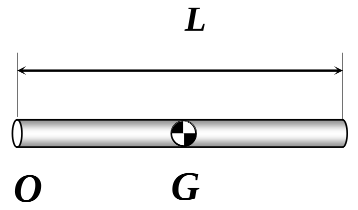
\includegraphics[width=0.75\linewidth]{moment-of-inertia-slender-rod-diagram} \\
  \(I_G = \frac{1}{12} m L^2\) \\
  \(I_O = \frac{1}{3} m L^2\)

  Disk or cylinder: \\
  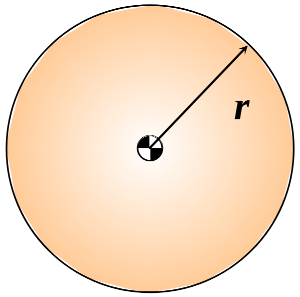
\includegraphics[width=0.3\linewidth]{moment-of-inertia-cylinder-or-disk-diagram} \\
  \(I_G = \frac{1}{2} m r^2\)

  Rectangular plate: \\
  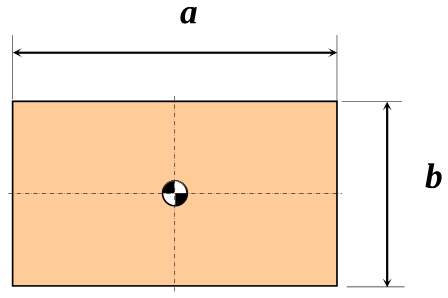
\includegraphics[width=0.6\linewidth]{moment-of-inertia-rectangular-plate-diagram} \\
  \(I_G = \frac{1}{12} m (a^2 + b^2)\)

  Ring: \\
  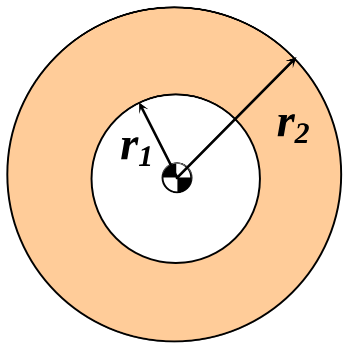
\includegraphics[width=0.4\linewidth]{moment-of-inertia-ring-diagram} \\
  \(I_G = \frac{1}{2} m (r_1^2 + r_2^2)\)

  Thin ring: \\
  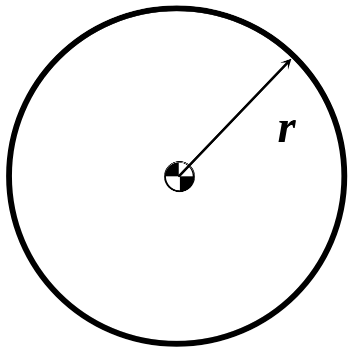
\includegraphics[width=0.4\linewidth]{moment-of-inertia-thin-ring-diagram} \\
  \(I_G = mr^2\)

  Semicircular plate: \\
  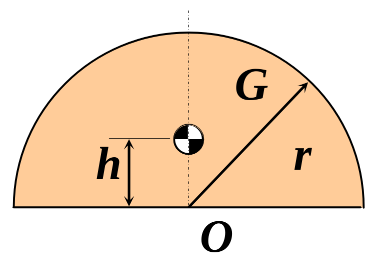
\includegraphics[width=0.4\linewidth]{moment-of-inertia-semicircular-plate-diagram} \\
  \(I_G = \frac{1}{2} mr^2\) \\
  \(h = \frac{4r}{3 \pi}\) \\
  \(I_O = \frac{1}{2} mr^2 - mh^2\)

  Parallel axis theorem: \\
  \(I_A = I_G + m |\vec{r}_{AG}|^2\)

  \section{Force analysis}

  \subsection{D'Alembert's Principle}
  \(\Diamond\) The direction of the inertial force (\(ma\)) or moment (\(I \alpha\)) is \textbf{opposite} to the direction of the resultant force or moment. \\
  \(\Diamond\) \textbf{Torque} (\(T\)) is not an inertial moment, so its direction does not need to be flipped. \\
  \(\Diamond\) The direction of the inertial acceleration (\(a\)) or angular velocity (\(\omega\)) is \textbf{opposite}
  to the direction of the acceleration force or angular velocity.

  \subsection{Steps}
  \(\Diamond\) Identify all \textbf{two-force members}. Two-force members are members with only two forces and no external force or torque. \\
  \(\Diamond\) For dynamic force analysis, \textbf{two-force members} must be \textbf{massless}. \\
  \(\Diamond\) For dynamic force analysis, \textbf{two-force members with mass} but with \textbf{1 net moment} can also be considered as a two force member. \\
  \(\Diamond\) Sliders and pin-in-slot joints always have a normal contact force acting opposite to the wall or slot they are resting on. \\
  \(\Diamond\) Draw applied forces and moments. Forces that have unknown directions are separated into the positive x and y components. \\
  \(\Diamond\) When moving from one link to another, remember to invert the direction of the forces acting on the other link. \\
  \(\Diamond\) \textbf{Two-force members} and \textbf{normal contact forces} have \textbf{known} directions. \\
  \(\Diamond\) Write the equilibrium equations for each free body. There is a total of \(3N\) equations for \(N\) bodies. \\
  \(\Diamond\) Solve the equations for the unknowns.




  \section{Maths}

  \subsection{Derivatives}

  Chain rule: \\
  \(\frac{dz}{dx} = \frac{dz}{dy} \cdot \frac{dy}{dx}\)

  Product rule: \\
  \(\frac{d}{dx} (u \cdot v) = \frac{du}{dx} \cdot v + u \cdot \frac{dv}{dx}\)

  Quotient rule: \\
  \(\frac{d}{dx} \left(\frac{f(x)}{g(x)} \right) = \frac{f'(x) g(x) - f(x) g'(x)}{g(x)^2}\)

  Standard derivatives: \\
  \(\frac{d}{dx} \left(\sin x \right) = \cos x\) \\
  \(\frac{d}{dx} \left(\cos x \right) = - \sin x\) \\
  \(\frac{d}{dx} \left(\arcsin x \right) = \frac{1}{\sqrt{1 - x^2}}\) \\
  \(\frac{d}{dx} \left(\arccos x \right) = - \frac{1}{\sqrt{1 - x^2}}\) \\
  \(\frac{d}{dx} \left(\arctan x \right) = \frac{1}{1 + x^2}\) \\
  \(\frac{d}{dx} \left(\csc x \right) = - \csc x \cot x\) \\
  \(\frac{d}{dx} \left(\sec x \right) = \sec x \tan x\)


  \subsection{Integrals}
  \(\int \sin x \, dx = - \cos x\) \\
  \(\int \cos x \, dx = \sin x\) \\
  \(\int \frac{1}{x^2 + a^2} \, dx = \frac{1}{a} \arctan \left(\frac{x}{a} \right)\) \\
  \(\int \frac{1}{\sqrt{a^2 - x^2}} \, dx = \arcsin \left(\frac{x}{a} \right)\) \\
  \(\int \frac{1}{x^2 - a^2} \, dx = \frac{1}{2a} \ln \left|\frac{x - a}{x + a} \right|\) \\
  \(\int \frac{1}{a^2 - x^2} \, dx = \frac{1}{2a} \ln \left|\frac{a + x}{a - x} \right|\) \\
  \(\int \frac{1}{\sqrt{x^2 - a^2}} \, dx = \ln \left|\sqrt{x^2 - a^2} + x \right|\) \\
  \(\int \tan x \, dx = \ln |\sec x|\) \\
  \(\int \cot x \, dx = \ln |\sin x|\) \\
  \(\int \csc x \, dx = - \ln |\csc x + \cot x|\) \\
  \(\int \sec x \, dx = - \ln |\sec x + \tan x|\)

  Integration by parts: \\
  \(\int u \, dv = uv - \int v \, du\)


  \subsection{Trigonometric identities}

  Quotient identities: \\
  \(\tan \theta = \frac{\sin \theta}{\cos \theta}\) \\
  \(\cot \theta = \frac{\cos \theta}{\sin \theta}\)

  Reciprocal identities: \\
  \(\sin \theta = \frac{1}{\csc \theta}\) \\
  \(\csc \theta = \frac{1}{\sin \theta}\) \\
  \(\cos \theta = \frac{1}{\sec \theta}\) \\
  \(\sec \theta = \frac{1}{\cos \theta}\) \\
  \(\tan \theta = \frac{1}{\cot \theta}\) \\
  \(\cot \theta = \frac{1}{\tan \theta}\)

  Pythagorean identities: \\
  \(\sin^2 \theta + \cos^2 \theta = 1\) \\
  \(\sec^2 \theta - \tan^2 \theta = 1\) \\
  \(\csc^2 \theta - \cot^2 \theta = 1\)

  Even/odd identities: \\
  \(\sin(- \theta) = - \sin \theta\) \\
  \(\cos (- \theta) = \cos \theta\) \\
  \(\tan(- \theta) = - \tan \theta\) \\
  \(\cot (- \theta) = - \cot \theta\) \\
  \(\csc(- \theta) = - \csc \theta\) \\
  \(\sec (- \theta) = \sec \theta\)

  Co-function identities: \\
  \(\sin \left(\frac{\pi}{2} - \theta \right) = \cos \theta\) \\
  \(\cos \left(\frac{\pi}{2} - \theta\right) = \sin \theta \) \\
  \(\tan \left(\frac{\pi}{2} - \theta \right) = \cot \theta\) \\
  \(\cot \left(\frac{\pi}{2} - \theta\right) = \tan \theta \) \\
  \(\csc \left(\frac{\pi}{2} - \theta \right) = \sec \theta\) \\
  \(\sec \left(\frac{\pi}{2} - \theta\right) = \csc \theta \) \\
  \(\frac{\pi}{2} \text{ radians} = 90^{\circ}\)

  Sum/difference identities: \\
  \(\sin (\theta \pm \phi) = \sin \theta \cos \phi \pm \cos \theta \sin \phi\) \\
  \(\cos (\theta \pm \phi) = \cos \theta \cos \phi \mp \sin \theta \sin \phi\) \\
  \(\tan (\theta \pm \phi) = \frac{\tan \theta \pm \tan \phi}{1 \mp \tan \theta \tan \phi}\)

  Double angle identities: \\
  \(\sin (2 \theta) = 2 \sin \theta \cos \theta\) \\
  \(\cos (2 \theta) = \cos^2 \theta - \sin^2 \theta\) \\
  \(\cos (2 \theta) = 2 \cos^2 \theta - 1\) \\
  \(\cos (2 \theta) = 1 - 2 \sin^2 \theta\) \\
  \(\tan (2 \theta) = \frac{2 \tan \theta}{1 - \tan^2 \theta}\)

  Half angle identities: \\
  \(\sin^2 \theta = \frac{1 - \cos (2 \theta)}{2}\) \\
  \(\cos^2 \theta = \frac{1 + \cos (2 \theta)}{2}\) \\
  \(\tan^2 \theta = \frac{1 - \cos (2 \theta)}{1 + \cos (2 \theta)}\)

  Sum to product of 2 angles: \\
  \(\sin \theta + \sin \phi = 2 \sin \left( \frac{\theta + \phi}{2} \right) \cos \left( \frac{\theta - \phi}{2} \right)\) \\
  \(\sin \theta - \sin \phi = 2 \cos \left( \frac{\theta + \phi}{2} \right) \sin \left( \frac{\theta - \phi}{2} \right)\) \\
  \(\cos \theta + \cos \phi = 2 \cos \left( \frac{\theta + \phi}{2} \right) \cos \left( \frac{\theta - \phi}{2} \right)\) \\
  \(\cos \theta - \cos \phi = - 2 \sin \left( \frac{\theta + \phi}{2} \right) \sin \left( \frac{\theta - \phi}{2} \right)\)

  Product to sum of 2 angles: \\
  \(\sin \theta \sin \phi = \frac{\cos (\theta - \phi) - \cos (\theta + \phi)}{2}\) \\
  \(\cos \theta \cos \phi = \frac{\cos (\theta - \phi) + \cos (\theta + \phi)}{2}\) \\
  \(\sin \theta \cos \phi = \frac{\sin (\theta + \phi) + \sin (\theta - \phi)}{2}\) \\
  \(\cos \theta \sin \phi = \frac{\sin (\theta + \phi) - \sin (\theta - \phi)}{2}\)

  Law of sines: \\
  \(\frac{a}{\sin A} = \frac{b}{\sin B} = \frac{c}{\sin C}\)

  Law of cosines: \\
  \(a^2 = b^2 + c^2 - 2bc \cos A\)

  Area of a triangle: \\
  \(A = \frac{1}{2} ab \sin C\)

\end{multicols*}
\end{document}
